%!TEX root=./main.tex
\section{Theory and Algorithms}
As explained in previous section, idea behind deconvolution of images, or any signal for that matter, is simple: divide fourier transform of the point spread function from fourier transform of image to get pure image object \textit{i.e.} from equation~\ref{eq:fourierconv}:
\begin{equation}
    \psi_t(x)= IFFT\{\Psi_i(\boldsymbol{k}) / H_o(\boldsymbol{k})\}
\end{equation}
where:
\begin{description}
    \item[IFFT] is inverse fourier transform operation
\end{description}
However there is one problem: transfer function $H_o(\boldsymbol{k})$ is oscillatory in nature and crosses zero several times (Figure~\ref{fig:ctffigure}).
Hence it results in division by zero error or amplification of noise.
Essentially whenever transfer function nears zero, that portion shall be avoided. 
To facilitate this one of the earliest approach was \textit{Parabola Approximation Method}\cite{OpdeBeeck1996}, where variation in defocus makes several `pass bands' which creates a linear region of contrast transfer in CTF.
As per previous reference, as linear contribution to HRTEM image comes from direct beam and diffracted beam, it can be shown that intensity of image in fourier space $I(\Psi(\boldsymbol{g}),\zeta)$ is proportional to:
\begin{equation}
    \frac{exp(-[\{\zeta - 0.5\lambda(g^2 + 2\boldsymbol{g.p})\}/\pi\alpha g])}{\pi\alpha g}exp(\iota 2 \pi C_s \lambda ^2\{g^2 + 3(p^2 + \boldsymbol{g.p})\}\{\zeta - 0.5 \lambda (g^2 + 2\boldsymbol{g.p})\})
    \label{eq:debeeckfourierI}
\end{equation}
where $\zeta$ represents inverse defocus in fourier space.
For parallel beams (\textit{i.e.} $\alpha = 0$), the first term in equation~\ref{eq:debeeckfourierI} reduces to Dirac delta function of form $\delta (\zeta - 0.5\lambda (g^2 + 2\boldsymbol{g.p}))$. 
ignoring the non-linear part this reduces to:
\begin{equation}
    \zeta = \pm 0.5\lambda g^2
\end{equation}
It is equivalent to propagation along Ewald sphere, where Ewald sphere is parabolic due to Fresnel approximation used in deriving the image intensity equation (see `Parxial approximation' of Helmholtz equation\cite{Hecht2002}). 
\begin{figure}[htp]
    \centering
    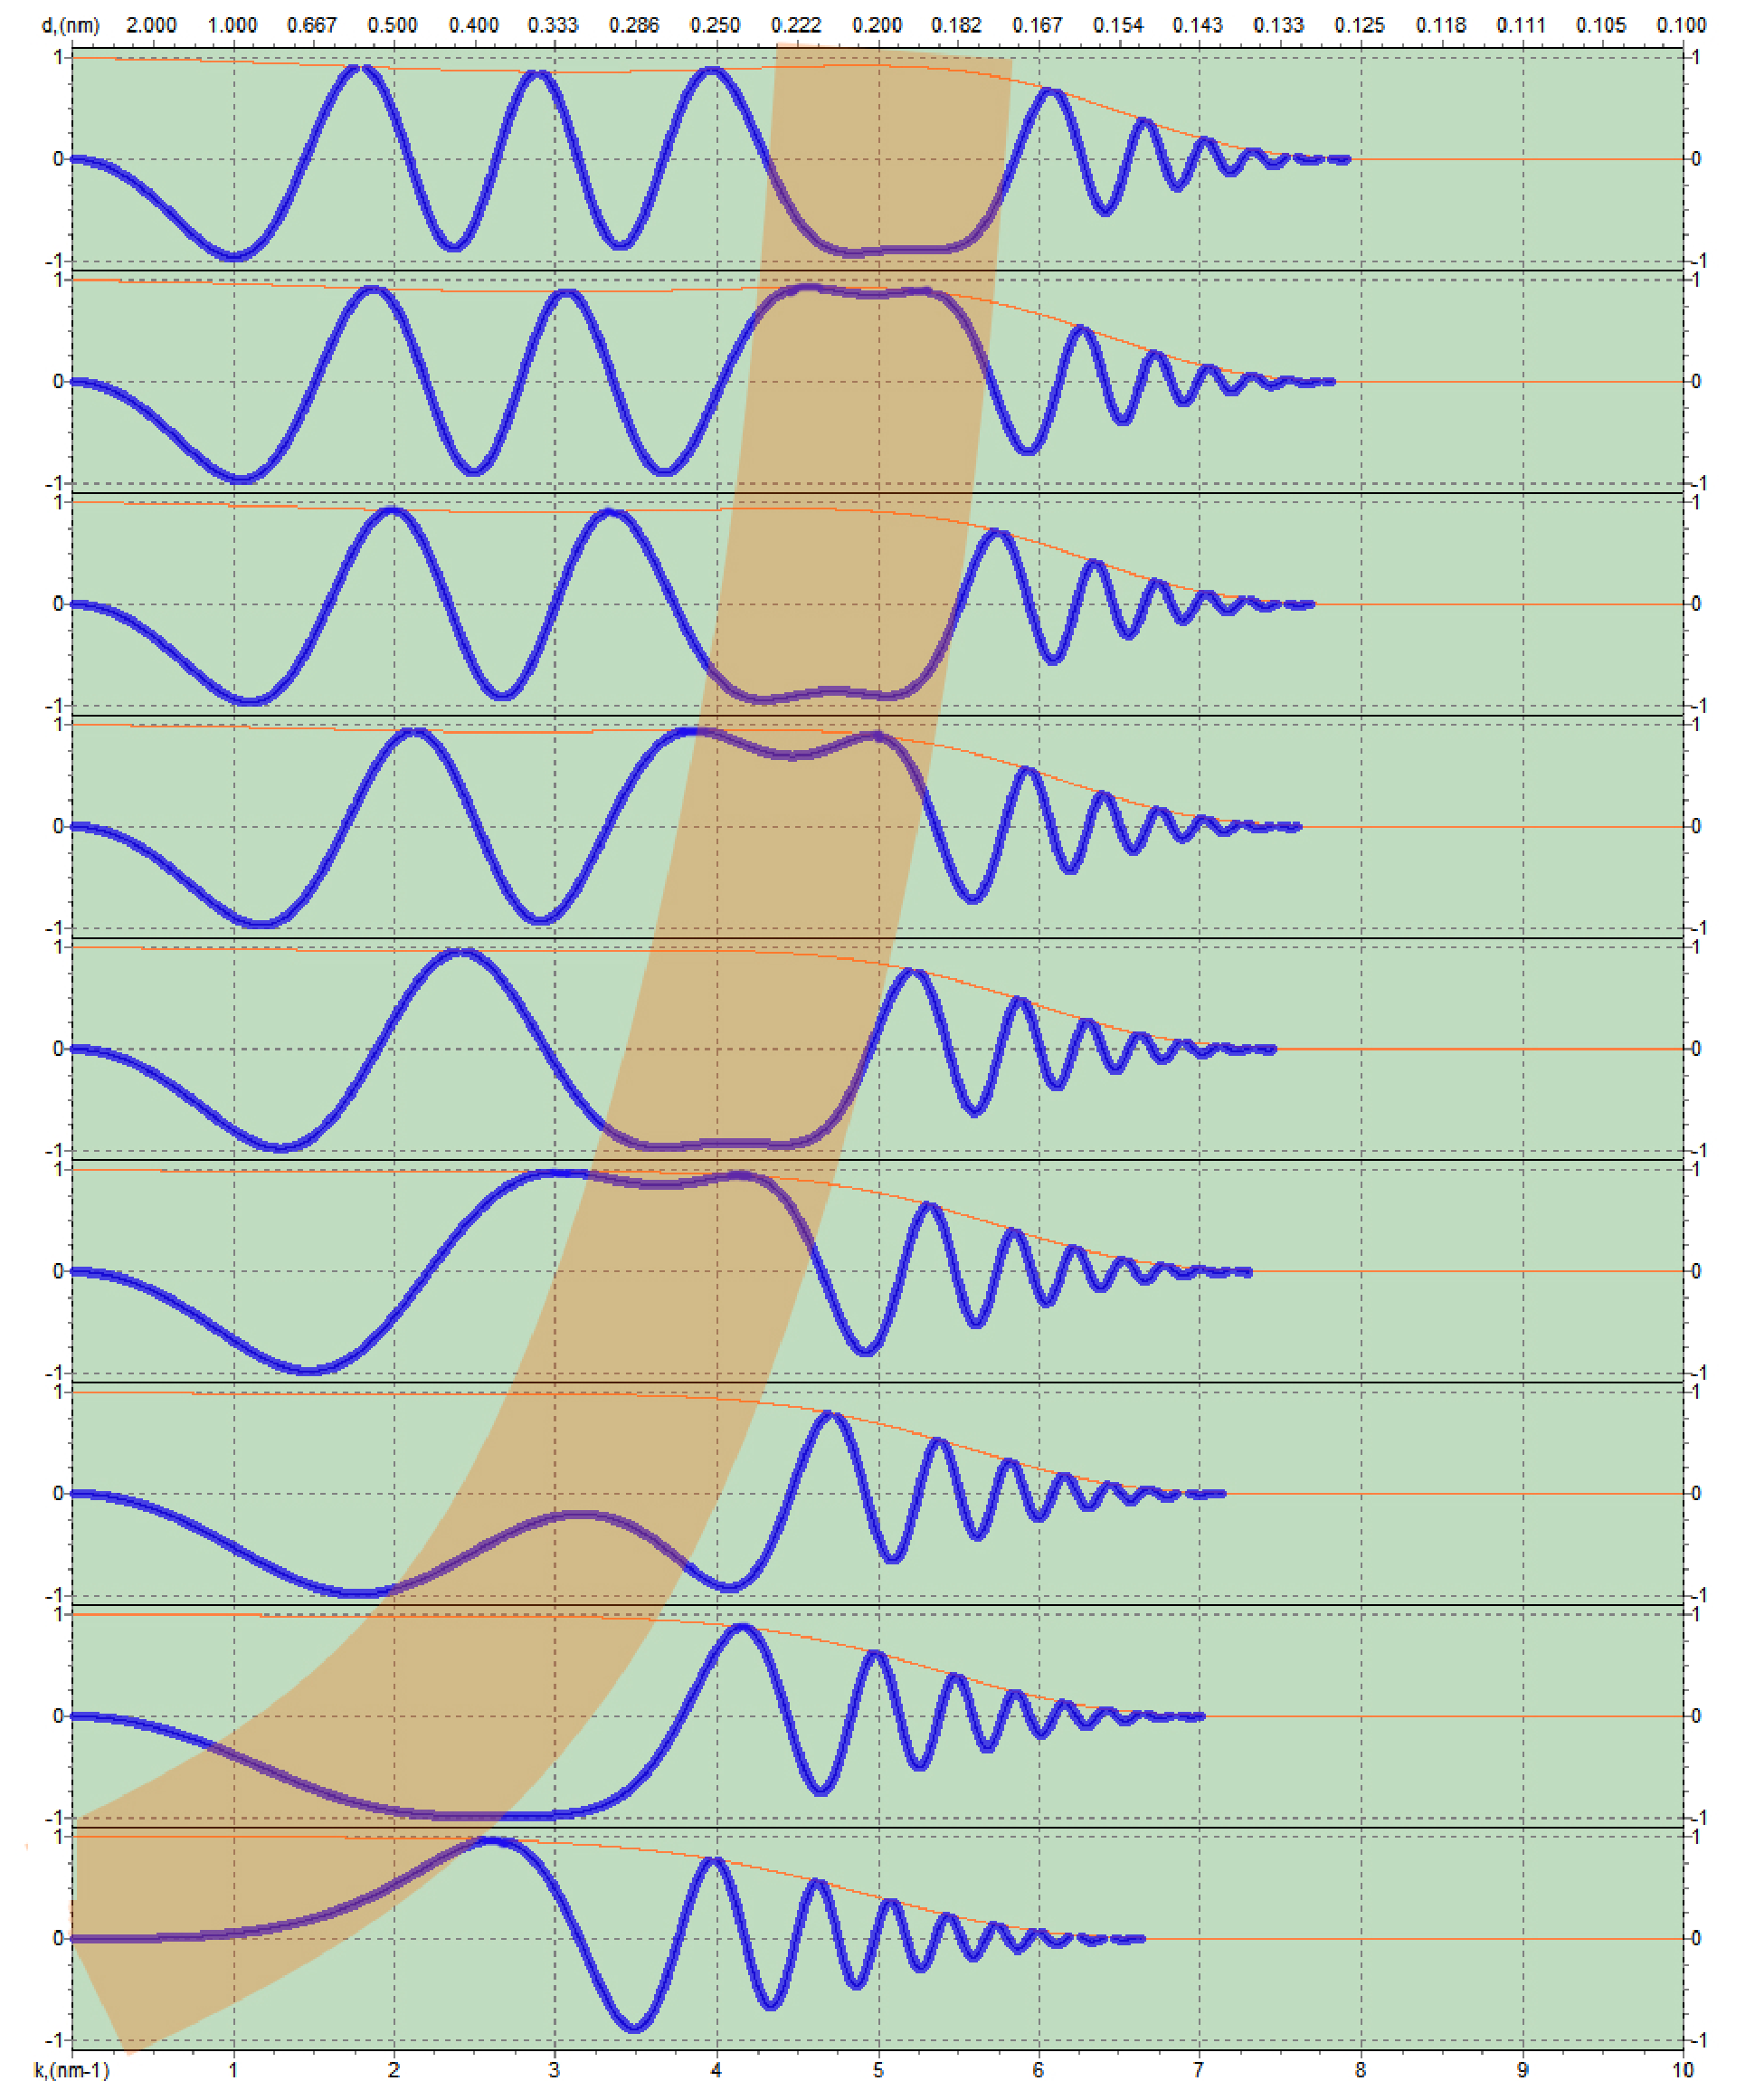
\includegraphics[width=\textwidth]{figures/ctfparabola.pdf}
    \caption{CTF showing propagation of linear pass bands with increase in defocus}
    \label{fig:ctfparabola}
\end{figure}


Hence all such pass bands (where $\boldsymbol{p}=0$ and $\boldsymbol{p}+\boldsymbol{g}=0$) lie on a paraboloid of a 3D Fourier transform of image stack, where 3rd dimension is defocus value.
Propagation of such pass bands with defocus in CTF is shown in Figure~\ref{fig:ctfparabola}. 
So basic principle is to get unaberrated linear contributions from various pass bands and stitch them together.


% \begin{wrapfigure}{}{\textwidth}
\begin{figure}[!ht]
    \centering
    \begin{tikzpicture}[node distance=2cm]
        \node(start) [startstop] {Start};
        \node(proc1) [process,below of = start] {Align TEM rigorously, specifically two fold astigmatism and coma};
        \node(in1) [io,below of = proc1] {Acquire images at different defocus values, preferably with constant difference between two consecutive defocus values};
        \node(proc2) [process,below of = in1] {Estimate defocus value for each image by fitting simulated CTF to FFT of image (fitting to Thon's rings)};
        \node(proc3) [process,below of = proc2] {Align each image within single pixel (sub-pixel alignment) and calculate largest common area for better result};
        \node(proc4) [process,below of = proc3] {Estimate noise by measuring standard deviation of any blank area in image (this step can be skipped initially)};
        \node(proc5) [process,below of = proc4] {Apply correction to each image using Wiener inverse filter to calculate phase and amplitude};
        \node(out1) [io,below of = proc5] {Write to Disk};
        \node(stop) [startstop, below of = out1] {Stop};
        % \node(dec1) [decision,below of = proc1,yshift=-0.5cm] {yes we can?};
        % \node(proc2) [process, right of = dec1,xshift=2cm] {here we go again};
        % \node(proc3) [process, below of = dec1,yshift=-0.5cm] {last chance};
        % \node(out1) [io, below of = proc3] {here it comes};
        % \node(end) [startstop, below of = out1] {Stop};
        \draw [arrow] (start)--(proc1);
        \draw [arrow] (proc1)--(in1);
        \draw [arrow] (in1)--(proc2);
        % \draw [arrow] (dec1)--node[anchor=west] {yes} (proc3);
        % \draw [arrow] (proc2)|-node[anchor=west] {no} (proc1);
        \draw [arrow] (proc2)--(proc3);
        \draw [arrow] (proc3)--(proc4);
        \draw [arrow] (proc4)--(proc5);
        \draw [arrow] (proc5)--(out1);
        \draw [arrow] (out1)--(stop);
    \end{tikzpicture}
    \caption{Basic schematic for Exit wave reconstruction}
    \label{fig:basic1}
\end{figure}
% \end{wrapfigure}


It can be demonstrated that above condition can be reduced to a special case called \textit{Wiener Inverse Filter}, before dwelling into detail, given here (Figure~\ref{fig:basic1}) is a simple algorithm for exit wave reconstruction.

\textbf{1. Alignment:}
Other than the usual TEM alignment, following things need to be paid special attention to: Condenser aperture, Objective astigmatism (2-fold), Coma.
Usually 2nd condenser aperture is a good compromise between intensity and coherence in HRTEM.
Two fold astigmatism can be removed from image by observing live FFT of amorphous background near region of interest on screen and compensating it with Objective stigmator till it is completely symmetric in both overfocus and underfocus condition.
Usually it can be corrected by measuring defocus in perpendicular directions and  numerically compensating it in Wave Aberration function\cite{meyer_symmetric}, but it has not been implemented yet in presented piece of code. 

It was found that coma correction yield better quality results than voltage centered images.
This can probably be explained by the fact that at high magnification, area of viewing is small hence small tilt in beam might not degrade image quality as much as the coma aberration.
Coma was corrected by rocking beam in x and y direction (under \textit{Maintenance \textgreater Alignment \textgreater Tilt X/Y}) while correcting tilt using \textit{bright tilt} in same direction, till FFT was same on both extremes of tilt.
Amplitude and frequency of rocking, and frame rate under CCD camera can be adjusted to aid if necessary. 

\textbf{2. Image Acquisition:}
Equation~\ref{eq:debeeckfourierI} was subjected to approximation that beam is parallel, \textit{i.e.} convergence angle is very low.
This can be ensured as following in JEOL microscopes by using $\alpha$1 mode (consult user manual on how to align it for the same).

Image drift shall be minimum while taking any images, it will not only give larger area to work upon (larger image area results in better less noisy FFT) but also drift results in streaking in images which looks like 2-fold astigmatism.
One of the simpler way to achieve above is to take a small video consisting for 20-30 frames and pick the frame that gives best results (a crude tool vid2img is provided for extracting frames from a video recorded from iTEM software).
Drift can be minimized by reducing exposure time as well, to compensate for decrease in intensity CCD camera's pixcels can be binned.
However such binning can be done later on numerically as well.

Once above is taken care of and image quality is of desired value, click 20-30 images at regular defocus, usually starting from slightly higher defocus value than Scherzer defocus as it is simpler to estimate defocus value from images in that region.
Pass bands can also be observed in live FFT which might aid in deciding the defocus interval.
Including small amount of amorphous carbon would be useful as well.

\textbf{3. Defocus estimation:}
If Spherical aberration coefficient of TEM is known accurately then defocus of any image can be determined by fitting minima of Thon's rings in FFT of images to the simulated CTF function.
For correct estimation of defocus value, CTF has to be simulated which requires accurate determination of spherical aberration coefficient.
For the microscope in use it was determined to be 0.95 mm, which is in close agreement with the quoted value, from the manufacturer, of 1.00 mm.
Spherical aberration coefficient was determined using tilt series cubic fit method.\cite{Koster1991} 
Defocus estimation by current method is slightly difficult if no amorphous carbon is present in image or if images are too close to exact defocus.
For defocus estimation \texttt{defocus\_esimation.m} GUI has been provided in current codes.

\begin{figure}
    \centering
    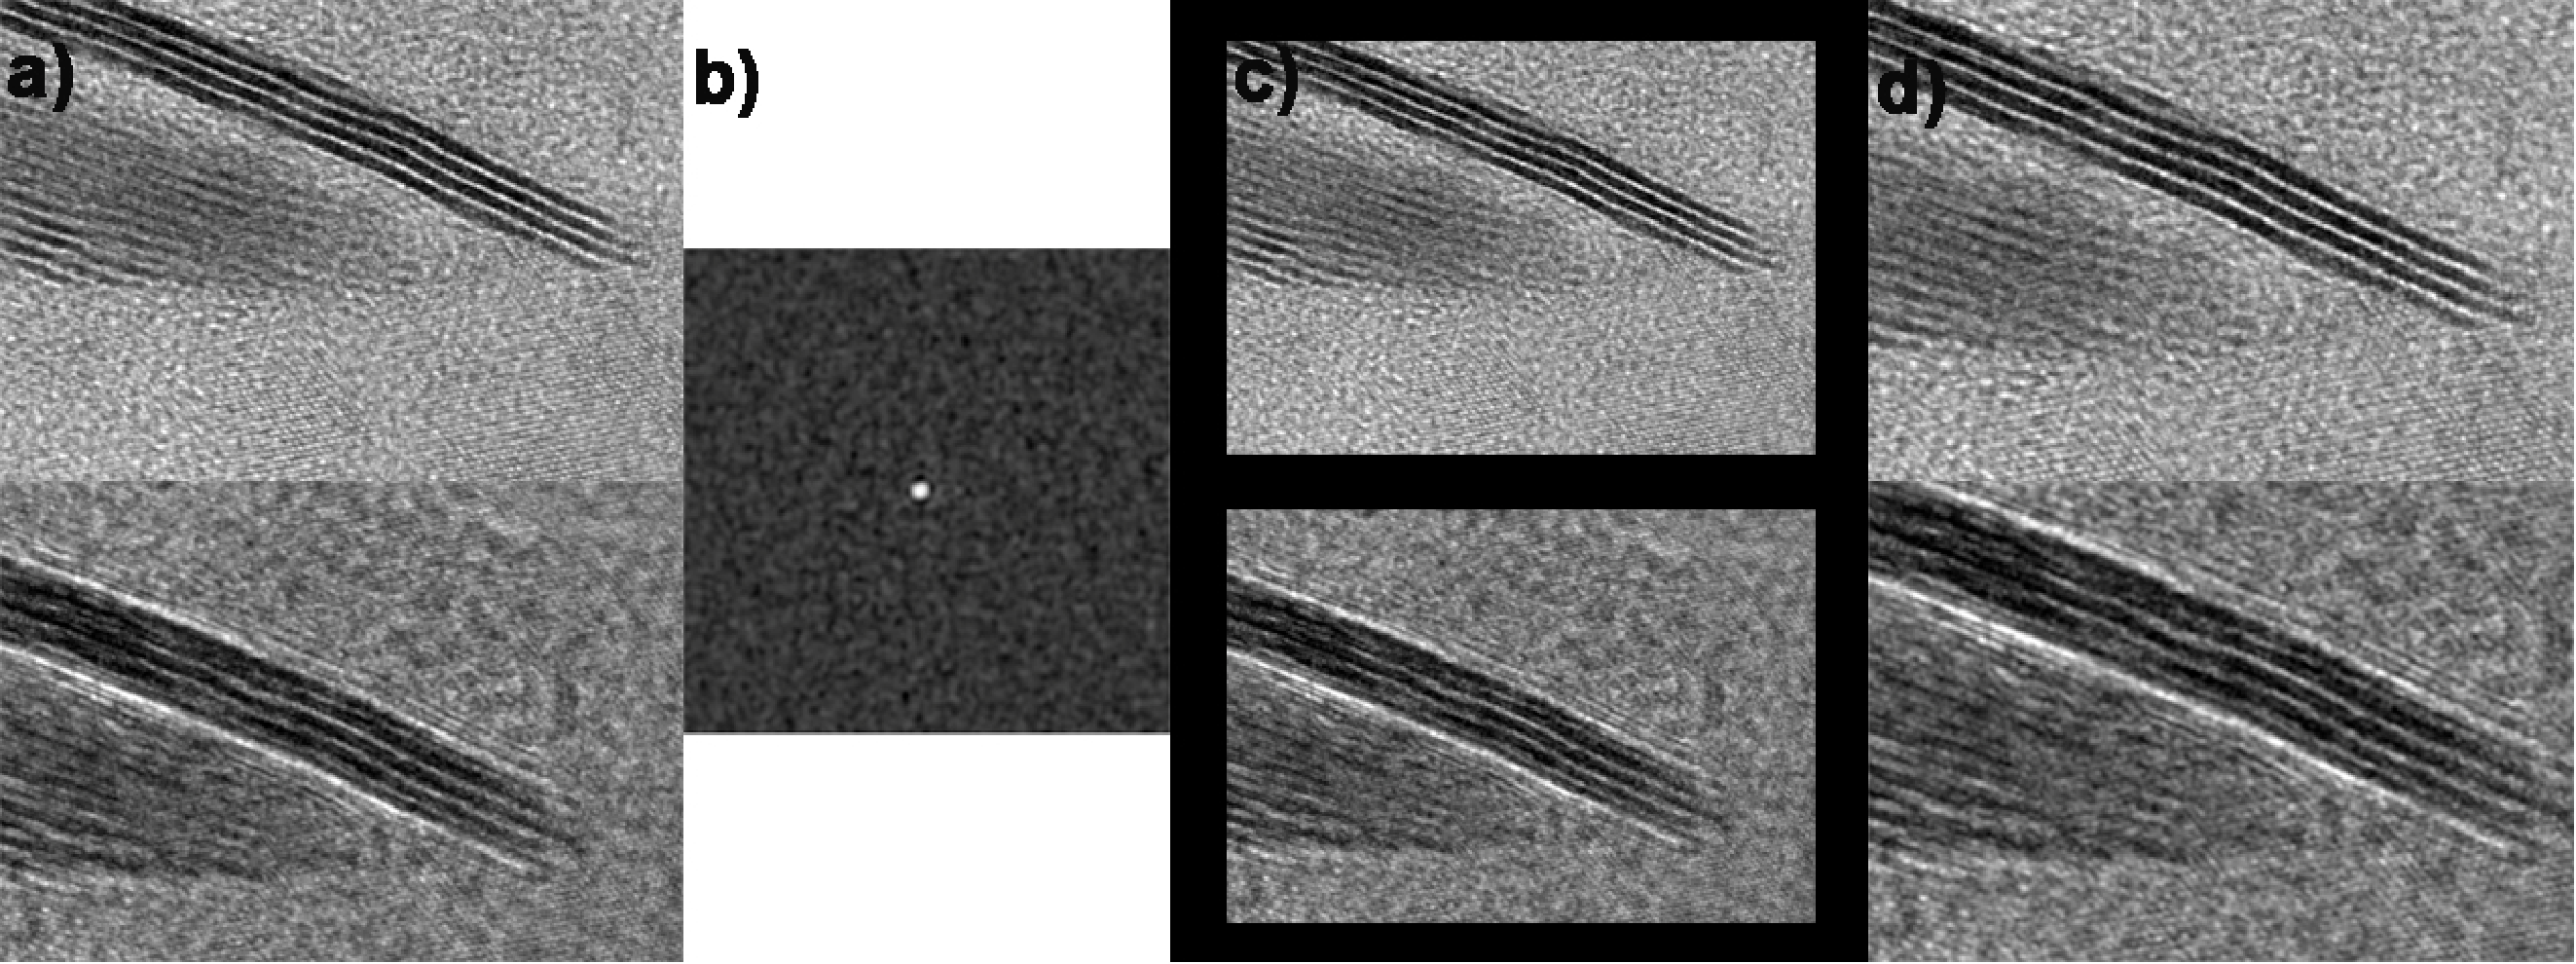
\includegraphics[width=\textwidth]{figures/LargestArea.pdf}
    \caption{Schematic representation of largest common image area selection and sub pixel alignment, a) initial images with large shift/drift, b) phase correlation peak between 2 images, c) padded and shifted images and d) common area of both images}
    \label{fig:subpixel}
\end{figure}

\textbf{4. Sub-pixel alignment:}
Sub-pixel alignment was divided into two parts: i) selection of largest common area in images, ii) sub-pixel alignment of the selected area.
To achieve this first phase correlation between all images were determined (\texttt{pcorr.m} file contains phase correlation code).
Following the determination of shift in each image, maximum shift was determined by summing all individual shifts (Figure~\ref{fig:subpixel}a and b).
To facilitate alignment of images, finally a blank padding was added to the images.
The width of padding was chosen to be slightly more than the total displacements among images.
All such shifted images were added in a single matrix, followed by binarization of the matrix, which then yields the mask which can be multiplied to each image, to get the common area from each image.

Area acquired as such is in fact all the images aligned up to a pixel.
For sub-pixel alignment, all the aligned images now were subjected to linear interpolation using \texttt{interp2} function of MATLAB.
Linear interpolation was chosen over cubic etc.\@, to minimize any induction of artifacts.
Procedure same as above was now applied to these extrapolated images, followed by restoration to original size.
Acquired images now were sub-pixel aligned.
This method was used over popular methods implemented in MATLAB, such as \texttt{imregcorr} or \texttt{dftregistration} \cite{Guizar-Sicairos:08}, as for TEM images, which are riddled with defocus artifacts none of the sub-pixel registration methods performed satisfactorily.

All the above mentioned code has been presented in file \texttt{im\_align\_self.m}.

\textbf{5. Determination of noise:}
Noise was determined to be the variation in intensity in a image without any thing under it, \textit{i.e.\@} any image of vacuum.
Noise level at present has to be given as separate variable in \texttt{waf\_recon.m} file.

\textbf{6. Wavefunction correction:}
To obtain the exit wave, Wiener inverse filter method was used, as described in literature. \cite{meyer_symmetric}
MATLAB implementation of Wiener inverse filter has been provided in \texttt{waf\_recon.m} file.
